\section{很多很多線段樹}

\begin{frame}{\ebtitle}
    \begin{figure}[h!]
        \begin{center}
            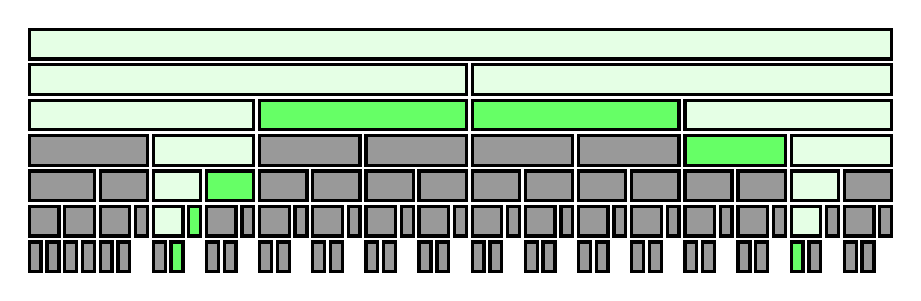
\begin{tikzpicture}[nodes = {transform shape}, scale=0.75]
                \pgfdeclarelayer{bg}
                \pgfsetlayers{bg, main}
                \tikzset{x={(0.1cm, 0cm)}, y={(0cm, 0.1cm)}}
            
                \draw [very thick, black, fill=white!90!green] (0, 0) rectangle (146, 5) node[black, midway, align=center] (nd0) {};
                \draw [very thick, black, fill=white!90!green] (0, -6) rectangle (74, -1) node[black, midway, align=center] (nd1) {};
                \draw [very thick, black, fill=white!90!green] (0, -12) rectangle (38, -7) node[black, midway, align=center] (nd3) {};
                \draw [very thick, black, fill=gray!80] (0, -18) rectangle (20, -13) node[black, midway, align=center] (nd7) {};
                \draw [very thick, black, fill=gray!80] (0, -24) rectangle (11, -19) node[black, midway, align=center] (nd15) {};
                \draw [very thick, black, fill=gray!80] (0, -30) rectangle (5, -25) node[black, midway, align=center] (nd31) {};
                \draw [very thick, black, fill=gray!80] (0, -36) rectangle (2, -31) node[black, midway, align=center] (nd63) {};
                \draw [very thick, black, fill=gray!80] (3, -36) rectangle (5, -31) node[black, midway, align=center] (nd64) {};
                \draw [very thick, black, fill=gray!80] (6, -30) rectangle (11, -25) node[black, midway, align=center] (nd32) {};
                \draw [very thick, black, fill=gray!80] (6, -36) rectangle (8, -31) node[black, midway, align=center] (nd65) {};
                \draw [very thick, black, fill=gray!80] (9, -36) rectangle (11, -31) node[black, midway, align=center] (nd66) {};
                \draw [very thick, black, fill=gray!80] (12, -24) rectangle (20, -19) node[black, midway, align=center] (nd16) {};
                \draw [very thick, black, fill=gray!80] (12, -30) rectangle (17, -25) node[black, midway, align=center] (nd33) {};
                \draw [very thick, black, fill=gray!80] (12, -36) rectangle (14, -31) node[black, midway, align=center] (nd67) {};
                \draw [very thick, black, fill=gray!80] (15, -36) rectangle (17, -31) node[black, midway, align=center] (nd68) {};
                \draw [very thick, black, fill=gray!80] (18, -30) rectangle (20, -25) node[black, midway, align=center] (nd34) {};
                \draw [very thick, black, fill=white!90!green] (21, -18) rectangle (38, -13) node[black, midway, align=center] (nd8) {};
                \draw [very thick, black, fill=white!90!green] (21, -24) rectangle (29, -19) node[black, midway, align=center] (nd17) {};
                \draw [very thick, black, fill=white!90!green] (21, -30) rectangle (26, -25) node[black, midway, align=center] (nd35) {};
                \draw [very thick, black, fill=gray!80] (21, -36) rectangle (23, -31) node[black, midway, align=center] (nd71) {};
                \draw [very thick, black, fill=white!40!green] (24, -36) rectangle (26, -31) node[black, midway, align=center] (nd72) {};
                \draw [very thick, black, fill=white!40!green] (27, -30) rectangle (29, -25) node[black, midway, align=center] (nd36) {};
                \draw [very thick, black, fill=white!40!green] (30, -24) rectangle (38, -19) node[black, midway, align=center] (nd18) {};
                \draw [very thick, black, fill=gray!80] (30, -30) rectangle (35, -25) node[black, midway, align=center] (nd37) {};
                \draw [very thick, black, fill=gray!80] (30, -36) rectangle (32, -31) node[black, midway, align=center] (nd75) {};
                \draw [very thick, black, fill=gray!80] (33, -36) rectangle (35, -31) node[black, midway, align=center] (nd76) {};
                \draw [very thick, black, fill=gray!80] (36, -30) rectangle (38, -25) node[black, midway, align=center] (nd38) {};
                \draw [very thick, black, fill=white!40!green] (39, -12) rectangle (74, -7) node[black, midway, align=center] (nd4) {};
                \draw [very thick, black, fill=gray!80] (39, -18) rectangle (56, -13) node[black, midway, align=center] (nd9) {};
                \draw [very thick, black, fill=gray!80] (39, -24) rectangle (47, -19) node[black, midway, align=center] (nd19) {};
                \draw [very thick, black, fill=gray!80] (39, -30) rectangle (44, -25) node[black, midway, align=center] (nd39) {};
                \draw [very thick, black, fill=gray!80] (39, -36) rectangle (41, -31) node[black, midway, align=center] (nd79) {};
                \draw [very thick, black, fill=gray!80] (42, -36) rectangle (44, -31) node[black, midway, align=center] (nd80) {};
                \draw [very thick, black, fill=gray!80] (45, -30) rectangle (47, -25) node[black, midway, align=center] (nd40) {};
                \draw [very thick, black, fill=gray!80] (48, -24) rectangle (56, -19) node[black, midway, align=center] (nd20) {};
                \draw [very thick, black, fill=gray!80] (48, -30) rectangle (53, -25) node[black, midway, align=center] (nd41) {};
                \draw [very thick, black, fill=gray!80] (48, -36) rectangle (50, -31) node[black, midway, align=center] (nd83) {};
                \draw [very thick, black, fill=gray!80] (51, -36) rectangle (53, -31) node[black, midway, align=center] (nd84) {};
                \draw [very thick, black, fill=gray!80] (54, -30) rectangle (56, -25) node[black, midway, align=center] (nd42) {};
                \draw [very thick, black, fill=gray!80] (57, -18) rectangle (74, -13) node[black, midway, align=center] (nd10) {};
                \draw [very thick, black, fill=gray!80] (57, -24) rectangle (65, -19) node[black, midway, align=center] (nd21) {};
                \draw [very thick, black, fill=gray!80] (57, -30) rectangle (62, -25) node[black, midway, align=center] (nd43) {};
                \draw [very thick, black, fill=gray!80] (57, -36) rectangle (59, -31) node[black, midway, align=center] (nd87) {};
                \draw [very thick, black, fill=gray!80] (60, -36) rectangle (62, -31) node[black, midway, align=center] (nd88) {};
                \draw [very thick, black, fill=gray!80] (63, -30) rectangle (65, -25) node[black, midway, align=center] (nd44) {};
                \draw [very thick, black, fill=gray!80] (66, -24) rectangle (74, -19) node[black, midway, align=center] (nd22) {};
                \draw [very thick, black, fill=gray!80] (66, -30) rectangle (71, -25) node[black, midway, align=center] (nd45) {};
                \draw [very thick, black, fill=gray!80] (66, -36) rectangle (68, -31) node[black, midway, align=center] (nd91) {};
                \draw [very thick, black, fill=gray!80] (69, -36) rectangle (71, -31) node[black, midway, align=center] (nd92) {};
                \draw [very thick, black, fill=gray!80] (72, -30) rectangle (74, -25) node[black, midway, align=center] (nd46) {};
                \draw [very thick, black, fill=white!90!green] (75, -6) rectangle (146, -1) node[black, midway, align=center] (nd2) {};
                \draw [very thick, black, fill=white!40!green] (75, -12) rectangle (110, -7) node[black, midway, align=center] (nd5) {};
                \draw [very thick, black, fill=gray!80] (75, -18) rectangle (92, -13) node[black, midway, align=center] (nd11) {};
                \draw [very thick, black, fill=gray!80] (75, -24) rectangle (83, -19) node[black, midway, align=center] (nd23) {};
                \draw [very thick, black, fill=gray!80] (75, -30) rectangle (80, -25) node[black, midway, align=center] (nd47) {};
                \draw [very thick, black, fill=gray!80] (75, -36) rectangle (77, -31) node[black, midway, align=center] (nd95) {};
                \draw [very thick, black, fill=gray!80] (78, -36) rectangle (80, -31) node[black, midway, align=center] (nd96) {};
                \draw [very thick, black, fill=gray!80] (81, -30) rectangle (83, -25) node[black, midway, align=center] (nd48) {};
                \draw [very thick, black, fill=gray!80] (84, -24) rectangle (92, -19) node[black, midway, align=center] (nd24) {};
                \draw [very thick, black, fill=gray!80] (84, -30) rectangle (89, -25) node[black, midway, align=center] (nd49) {};
                \draw [very thick, black, fill=gray!80] (84, -36) rectangle (86, -31) node[black, midway, align=center] (nd99) {};
                \draw [very thick, black, fill=gray!80] (87, -36) rectangle (89, -31) node[black, midway, align=center] (nd100) {};
                \draw [very thick, black, fill=gray!80] (90, -30) rectangle (92, -25) node[black, midway, align=center] (nd50) {};
                \draw [very thick, black, fill=gray!80] (93, -18) rectangle (110, -13) node[black, midway, align=center] (nd12) {};
                \draw [very thick, black, fill=gray!80] (93, -24) rectangle (101, -19) node[black, midway, align=center] (nd25) {};
                \draw [very thick, black, fill=gray!80] (93, -30) rectangle (98, -25) node[black, midway, align=center] (nd51) {};
                \draw [very thick, black, fill=gray!80] (93, -36) rectangle (95, -31) node[black, midway, align=center] (nd103) {};
                \draw [very thick, black, fill=gray!80] (96, -36) rectangle (98, -31) node[black, midway, align=center] (nd104) {};
                \draw [very thick, black, fill=gray!80] (99, -30) rectangle (101, -25) node[black, midway, align=center] (nd52) {};
                \draw [very thick, black, fill=gray!80] (102, -24) rectangle (110, -19) node[black, midway, align=center] (nd26) {};
                \draw [very thick, black, fill=gray!80] (102, -30) rectangle (107, -25) node[black, midway, align=center] (nd53) {};
                \draw [very thick, black, fill=gray!80] (102, -36) rectangle (104, -31) node[black, midway, align=center] (nd107) {};
                \draw [very thick, black, fill=gray!80] (105, -36) rectangle (107, -31) node[black, midway, align=center] (nd108) {};
                \draw [very thick, black, fill=gray!80] (108, -30) rectangle (110, -25) node[black, midway, align=center] (nd54) {};
                \draw [very thick, black, fill=white!90!green] (111, -12) rectangle (146, -7) node[black, midway, align=center] (nd6) {};
                \draw [very thick, black, fill=white!40!green] (111, -18) rectangle (128, -13) node[black, midway, align=center] (nd13) {};
                \draw [very thick, black, fill=gray!80] (111, -24) rectangle (119, -19) node[black, midway, align=center] (nd27) {};
                \draw [very thick, black, fill=gray!80] (111, -30) rectangle (116, -25) node[black, midway, align=center] (nd55) {};
                \draw [very thick, black, fill=gray!80] (111, -36) rectangle (113, -31) node[black, midway, align=center] (nd111) {};
                \draw [very thick, black, fill=gray!80] (114, -36) rectangle (116, -31) node[black, midway, align=center] (nd112) {};
                \draw [very thick, black, fill=gray!80] (117, -30) rectangle (119, -25) node[black, midway, align=center] (nd56) {};
                \draw [very thick, black, fill=gray!80] (120, -24) rectangle (128, -19) node[black, midway, align=center] (nd28) {};
                \draw [very thick, black, fill=gray!80] (120, -30) rectangle (125, -25) node[black, midway, align=center] (nd57) {};
                \draw [very thick, black, fill=gray!80] (120, -36) rectangle (122, -31) node[black, midway, align=center] (nd115) {};
                \draw [very thick, black, fill=gray!80] (123, -36) rectangle (125, -31) node[black, midway, align=center] (nd116) {};
                \draw [very thick, black, fill=gray!80] (126, -30) rectangle (128, -25) node[black, midway, align=center] (nd58) {};
                \draw [very thick, black, fill=white!90!green] (129, -18) rectangle (146, -13) node[black, midway, align=center] (nd14) {};
                \draw [very thick, black, fill=white!90!green] (129, -24) rectangle (137, -19) node[black, midway, align=center] (nd29) {};
                \draw [very thick, black, fill=white!90!green] (129, -30) rectangle (134, -25) node[black, midway, align=center] (nd59) {};
                \draw [very thick, black, fill=white!40!green] (129, -36) rectangle (131, -31) node[black, midway, align=center] (nd119) {};
                \draw [very thick, black, fill=gray!80] (132, -36) rectangle (134, -31) node[black, midway, align=center] (nd120) {};
                \draw [very thick, black, fill=gray!80] (135, -30) rectangle (137, -25) node[black, midway, align=center] (nd60) {};
                \draw [very thick, black, fill=gray!80] (138, -24) rectangle (146, -19) node[black, midway, align=center] (nd30) {};
                \draw [very thick, black, fill=gray!80] (138, -30) rectangle (143, -25) node[black, midway, align=center] (nd61) {};
                \draw [very thick, black, fill=gray!80] (138, -36) rectangle (140, -31) node[black, midway, align=center] (nd123) {};
                \draw [very thick, black, fill=gray!80] (141, -36) rectangle (143, -31) node[black, midway, align=center] (nd124) {};
                \draw [very thick, black, fill=gray!80] (144, -30) rectangle (146, -25) node[black, midway, align=center] (nd62) {};
            \end{tikzpicture}
        \end{center}
        \caption{$N = 49$,區間查詢 $[9, 44]$(Source:2024 基礎資結投影片)}
    \end{figure}
\end{frame}

\begin{frame}{\btitle{前言}}
    你一定寫過線段樹!

    線段樹普及,大家都會用線段樹砸區間操作 \\
    你都用線段樹做過什麼事情?
\end{frame}

\begin{frame}{\btitle{前言}}
    \begin{itemize}
        \item \tikzoverlay{nd0}{}區間求和、極值、最大公因數
        \item \tikzoverlay{nd1}{}單點修改、區間加值
        \item \tikzoverlay{nd2}{}歷史版本的區間和
        \item \tikzoverlay{nd3}{}區間最大連續和
        \item \tikzoverlay{nd4}{}區間 MEX、矩形覆蓋面積
        \item \tikzoverlay{nd5}{}靜態區間和 \brilliance{blunder}
    \end{itemize}

    \begin{tikzpicture}[remember picture, overlay]
        \node[right=6cm of nd0, anchor=base west] {(一般線段樹)};
        \node[right=6cm of nd1, anchor=base west] {(懶人標記)};
        \node[right=6cm of nd2, anchor=base west] {(持久化)};
        \node[right=6cm of nd3, anchor=base west] {(分治)};
        \node[right=6cm of nd4, anchor=base west] {(離線、掃描線)};
        \node[right=6cm of nd5, anchor=base west] {(拜託不要)};
    \end{tikzpicture}
\end{frame}

\begin{frame}{\btitle{前言}}
    不只是區間詢問,線段樹可以有更多花樣!

    \begin{itemize}
        \item 李超線段樹
        \item 時間線段樹
        \item 線段樹優化建圖
    \end{itemize}
\end{frame}


\subsection{李超線段樹}

\begin{frame}{\ectitle}
    \begin{problem}[動態凸包]
        現在有 $Q$ 個操作,每個操作會是以下兩種中的一種:

        \begin{itemize}
            \item 加入一條直線 $y = mx + k$
            \item 詢問在 $x = t$ 處最大的 $y$ 值
        \end{itemize}

        \begin{itemize}
            \item $1\le Q \le 10^5$
            \item $|m|, |k| \le 10^9$
            \item $1 \le t \le 10^5$
        \end{itemize}
    \end{problem}
\end{frame}

\begin{frame}{\ectitle}
    用 set 維護上凸包上的線段,維護線段控制的左右界,每次加入直線先搜他控制的區間,往左右殺掉其他線段,查詢的時候二分搜是哪條線段代值進去。注意 iterator 使用、全整求線交點......

    太麻煩了,而且常數不小\sout{,而且我沒寫過} \\
    有沒有簡單一點的辦法?
\end{frame}

\begin{frame}{\ectitle}
    李超線段樹:
    \begin{itemize}
        \item 對要查詢的\yum{值域}開線段樹,葉子代表單一一個 $x$ 的值
        \item 每個節點存\yum{一條}對\yum{中點}來說 $y$ 最大的直線
        \begin{itemize}
            \item 對中點一定是有用的
            \item 可能還對這個區間的其他一部分有用
        \end{itemize}
    \end{itemize}
\end{frame}

\begin{frame}{\ctitle{插入直線}}
    原本節點上有一條直線 \\
    這次詢問想插入另外一條直線

    一個節點只能存一條線
    誰要留下來?另一條線要去哪裡?
\end{frame}

\begin{frame}{\ctitle{插入直線}}
    \only<1> {
        \begin{centikz}
            \draw[color=gray, dashed] (-5, 0) -- (-5, 5);
            \draw[color=gray, dashed] ( 0, 0) -- ( 0, 5);
            \draw[color=gray, dashed] ( 5, 0) -- ( 5, 5);
            \node[color=gray, anchor=north] at (-5, -0.2) {$L$};
            \node[color=gray, anchor=north] at ( 0, -0.2) {$M = \frac{L + R}{2}$};
            \node[color=gray, anchor=north] at ( 5, -0.2) {$R$};
            \draw[color=black, very thick] plot[domain=-5:5] (\x,{0.3 * \x + 2.8});
            \draw[color=black, very thick] plot[domain=-5:5] (\x,{-0.2 * \x + 2.1});
        \end{centikz}
    }

    \only<2> {
        \begin{centikz}
            \draw[color=gray, dashed] (-5, 0) -- (-5, 5);
            \draw[color=gray, dashed] ( 0, 0) -- ( 0, 5);
            \draw[color=gray, dashed] ( 5, 0) -- ( 5, 5);
            \node[color=gray, anchor=north] at (-5, -0.2) {$L$};
            \node[color=gray, anchor=north] at ( 0, -0.2) {$M = \frac{L + R}{2}$};
            \node[color=gray, anchor=north] at ( 5, -0.2) {$R$};
            \draw[color=black, very thick] plot[domain=-5:5] (\x,{-0.2 * \x + 2.1});
            \draw[color=Lime, very thick] plot[domain=-5:5] (\x,{0.3 * \x + 2.8});
            \node[anchor=south west] at (0, 3) {\brilliance{best}};
        \end{centikz}
    }

    \only<3> {
        \begin{centikz}
            \draw[color=gray, dashed] (-5, 0) -- (-5, 5);
            \draw[color=gray, dashed] ( 0, 0) -- ( 0, 5);
            \draw[color=gray, dashed] ( 5, 0) -- ( 5, 5);
            \node[color=gray, anchor=north] at (-5, -0.2) {$L$};
            \node[color=gray, anchor=north] at ( 0, -0.2) {$M = \frac{L + R}{2}$};
            \node[color=gray, anchor=north] at ( 5, -0.2) {$R$};
            
            \draw[color=DarkSeaGreen, very thick] plot[domain=-5:-1.4] (\x,{-0.2 * \x + 2.1});
            \draw[color=Red, very thick] plot[domain=-1.4:5] (\x,{-0.2 * \x + 2.1});
            \node[anchor=south] at (-3.2, 2.84) {\brilliance{good}};
            \node[anchor=south] at (2.5, 1.7) {\brilliance{incorrect}};
            
            \draw[color=Lime, very thick] plot[domain=-5:5] (\x,{0.3 * \x + 2.8});
            \node[anchor=south west] at (0, 3) {\brilliance{best}};
        \end{centikz}
    }
\end{frame}

\begin{frame}{\ctitle{插入直線}}
    \only<1> {
        \begin{centikz}
            \draw[color=gray, dashed] (-5, 0) -- (-5, 5);
            \draw[color=gray, dashed] ( 0, 0) -- ( 0, 5);
            \draw[color=gray, dashed] ( 5, 0) -- ( 5, 5);
            \node[color=gray, anchor=north] at (-5, -0.2) {$L$};
            \node[color=gray, anchor=north] at ( 0, -0.2) {$M = \frac{L + R}{2}$};
            \node[color=gray, anchor=north] at ( 5, -0.2) {$R$};
            \draw[color=black, very thick] plot[domain=-5:5] (\x,{0.3 * \x + 2.1});
            \draw[color=black, very thick] plot[domain=-5:5] (\x,{-0.2 * \x + 2.8});
        \end{centikz}
    }

    \only<2> {
        \begin{centikz}
            \draw[color=gray, dashed] (-5, 0) -- (-5, 5);
            \draw[color=gray, dashed] ( 0, 0) -- ( 0, 5);
            \draw[color=gray, dashed] ( 5, 0) -- ( 5, 5);
            \node[color=gray, anchor=north] at (-5, -0.2) {$L$};
            \node[color=gray, anchor=north] at ( 0, -0.2) {$M = \frac{L + R}{2}$};
            \node[color=gray, anchor=north] at ( 5, -0.2) {$R$};
            \draw[color=black, very thick] plot[domain=-5:5] (\x,{0.3 * \x + 2.1});
            \draw[color=Lime, very thick] plot[domain=-5:5] (\x,{-0.2 * \x + 2.8});
            \node[anchor=south west] at (0, 2.8) {\brilliance{best}};
        \end{centikz}
    }

    \only<3> {
        \begin{centikz}
            \draw[color=gray, dashed] (-5, 0) -- (-5, 5);
            \draw[color=gray, dashed] ( 0, 0) -- ( 0, 5);
            \draw[color=gray, dashed] ( 5, 0) -- ( 5, 5);
            \node[color=gray, anchor=north] at (-5, -0.2) {$L$};
            \node[color=gray, anchor=north] at ( 0, -0.2) {$M = \frac{L + R}{2}$};
            \node[color=gray, anchor=north] at ( 5, -0.2) {$R$};

            \draw[color=Red, very thick] plot[domain=-5:1.4] (\x,{0.3 * \x + 2.1});
            \draw[color=DarkSeaGreen, very thick] plot[domain=1.4:5] (\x,{0.3 * \x + 2.1});
            \node[anchor=south] at (-2.5, 1.45) {\brilliance{incorrect}};
            \node[anchor=south] at (3.2, 3.16) {\brilliance{good}};

            \draw[color=Lime, very thick] plot[domain=-5:5] (\x,{-0.2 * \x + 2.8});
            \node[anchor=south west] at (0, 2.8) {\brilliance{best}};
        \end{centikz}
    }
\end{frame}

\begin{frame}{\ctitle{插入直線}}
    一條直線在中點輸掉之後不能直接扔掉,因為他還沒輸光,區間內某些 $x$ 的範圍可能還需要他

    在中點輸掉的話,一定也會在左右其中一邊輸光 \\
    只有其中一邊可能還會需要用到這條直線,遞迴把他交給線段樹上那半邊的子樹處置,另外半邊已經不需要他了

    到葉子還輸的話那這條線徹底不會被任何人需要
\end{frame}

\begin{frame}{\ctitle{插入直線}}
    \only<1> {
        \begin{centikz}
            \draw[color=gray, dashed] (-5, 0) -- (-5, 5);
            \draw[color=gray, dashed] ( 0, 0) -- ( 0, 5);
            \draw[color=gray, dashed] ( 5, 0) -- ( 5, 5);
            \node[color=gray, anchor=north] at (-5, -0.2) {$L$};
            \node[color=gray, anchor=north] at ( 0, -0.2) {$M = \frac{L + R}{2}$};
            \node[color=gray, anchor=north] at ( 5, -0.2) {$R$};
            \draw[color=black, very thick] plot[domain=-5:5] (\x,{0.3 * \x + 2.8});
            \draw[color=black, very thick] plot[domain=-5:5] (\x,{-0.2 * \x + 2.1});
        \end{centikz}
    }

    \only<2> {
        \begin{centikz}
            \draw[color=gray, dashed] (-5, 0) -- (-5, 5);
            \draw[color=gray, dashed] ( 0, 0) -- ( 0, 5);
            \draw[color=gray, dashed] ( 5, 0) -- ( 5, 5);
            \node[color=gray, anchor=north] at (-5, -0.2) {$L$};
            \node[color=gray, anchor=north] at ( 0, -0.2) {$M = \frac{L + R}{2}$};
            \node[color=gray, anchor=north] at ( 5, -0.2) {$R$};
            \draw[color=DarkSeaGreen, very thick] plot[domain=-5:0] (\x,{-0.2 * \x + 2.1});
            \draw[color=Lime, very thick] plot[domain=-5:5] (\x,{0.3 * \x + 2.8});
            \node[anchor=south west] at (0, 3) {\brilliance{best}};
            \node[anchor=south] at (-2.5, 2.7) {\brilliance{forced}};
        \end{centikz}
    }

    \only<3> {
        \begin{centikz}
            \draw[color=gray, dashed] (-5, 0) -- (-5, 5);
            \draw[color=gray, dashed] ( 0, 0) -- ( 0, 5);
            \draw[color=gray, dashed] ( 5, 0) -- ( 5, 5);
            \node[color=gray, anchor=north] at (-5, -0.2) {$L$};
            \node[color=gray, anchor=north] at ( 0, -0.2) {$M = \frac{L + R}{2}$};
            \node[color=gray, anchor=north] at ( 5, -0.2) {$R$};
            \draw[color=black, very thick] plot[domain=-5:5] (\x,{0.3 * \x + 2.1});
            \draw[color=black, very thick] plot[domain=-5:5] (\x,{-0.2 * \x + 2.8});
        \end{centikz}
    }

    \only<4> {
        \begin{centikz}
            \draw[color=gray, dashed] (-5, 0) -- (-5, 5);
            \draw[color=gray, dashed] ( 0, 0) -- ( 0, 5);
            \draw[color=gray, dashed] ( 5, 0) -- ( 5, 5);
            \node[color=gray, anchor=north] at (-5, -0.2) {$L$};
            \node[color=gray, anchor=north] at ( 0, -0.2) {$M = \frac{L + R}{2}$};
            \node[color=gray, anchor=north] at ( 5, -0.2) {$R$};
            \draw[color=DarkSeaGreen, very thick] plot[domain=0:5] (\x,{0.3 * \x + 2.1});
            \draw[color=Lime, very thick] plot[domain=-5:5] (\x,{-0.2 * \x + 2.8});
            \node[anchor=south west] at (0, 2.8) {\brilliance{best}};
            \node[anchor=south] at (2.5, 2.95) {\brilliance{forced}};
        \end{centikz}
    }
\end{frame}

\begin{frame}{\ctitle{插入直線}}
    從根節點出發,到葉節點為止:

    \begin{itemize}
        \item 代中點 $x$ 座標比較兩條直線,贏家留在節點上
        \item 比較兩條直線的斜率
        \begin{itemize}
            \item 如果贏家的斜率比較\strong{大},輸家往\strong{左}子樹遞迴插入
            \item 如果贏家的斜率比較\strong{小},輸家往\strong{右}子樹遞迴插入
        \end{itemize}
    \end{itemize}

    一直往子樹丟包直線\\
    時間複雜度 $O(\text{線段樹高}) = O(\log N)$
\end{frame}

\begin{frame}{\ctitle{單點查詢}}
    直線被扔到隔壁節點,代表這個範圍的 $x$ 全都用不到這條直線 \\
    一個 $x$ 可能用到的直線,都存在他的祖先們身上

    \begin{itemize}
        \item 找到代表這個 $x$ 值的葉子
        \item 檢查所有祖先存的直線,每個都代一次,回答最大的 $y$
    \end{itemize}

    時間複雜度 $O(\text{線段樹高}) = O(\log N)$
\end{frame}

\begin{frame}[fragile]{\ctitle{實做}}
    包裝直線作為函數使用
    
    \begin{minted}{cpp}
        struct Line {
            int a, b;  // y = ax + b
            Line(int _a = 0, int _b = 0): a(_a), b(_b) {}
            int operator()(int x) { return a * x + b; }
        };
    \end{minted}
\end{frame}

\begin{frame}[fragile]{\ctitle{實做}}
    插入直線

    \begin{itemize}
        \item 代中點 $x$ 座標比較兩條直線,贏家留在節點上
        \item 比較兩條直線的斜率
        \item 遞迴插入
    \end{itemize}
    
    \begin{minted}{cpp}
        void insert(int id, int l, int r, Line ln) {
            int m = (l + r) / 2;
            if(lns[id](m) < ln(m)) swap(lns[id], ln);
            if(l == r) return;
            if(lns[id].a > ln.a) insert(L(id), l, m, ln);
            else insert(R(id), m + 1, r, ln);
        }
    \end{minted}
\end{frame}

\begin{frame}[fragile]{\ctitle{實做}}
    單點查詢

    \begin{itemize}
        \item 找到代表這個 $x$ 值的葉子
        \item 檢查所有祖先存的直線,每個都代一次,回答最大的 $y$
    \end{itemize}
    
    \begin{minted}{cpp}
        int qry(int id, int l, int r, int x) {
            int m = (l + r) / 2;
            int res = lns[id](x);
            if(l == r) return res;
            if(x <= m) res = max(res, qry(L(id), l, m, x));
            else res = max(res, qry(R(id), m + 1, r, x));
            return res;
        }
    \end{minted}
\end{frame}

\begin{frame}{\ctitle{座標壓縮}}
    \begin{problem}[Line Add Get Min,Library Checker]
        你有 $N$ 條直線 $y = a_i x + b_i$。請你處理 $Q$ 個詢問:

        \begin{itemize}
            \item 加入一條直線 $y = ax + b$
            \item 詢問 $x = p$ 處最小的 $y$ 值
        \end{itemize}

        \begin{itemize}
            \item $1 \le N, Q \le 2 \times 10^5$
            \item $|a_i|, |p| \le 10^9$ \only<2>{\yum{???!!}}
            \item $|b_i| \le 10^{18}$
        \end{itemize}
    \end{problem}
\end{frame}

\begin{frame}{\ctitle{座標壓縮}}
    剛剛對 $x$ 的值域 $1, 2, \dots, 10^5$ 開線段樹

    現在事先收集會被詢問到的 $x$ 座標 \\
    對會被問到的 $x$ 開線段樹

    詢問是浮點數的時候也可以
\end{frame}

\begin{frame}{\ctitle{座標壓縮}}
    如果事先不知道詢問位置呢?

    \only<2> {
        動態開點,用不到的節點不要理他
    }
\end{frame}

\begin{frame}{\ctitle{插入線段}}
    如果插入的不是直線,而是有左右範圍限制的線段呢?

    \todo 插圖
\end{frame}

\begin{frame}{\ctitle{插入線段}}
    一般線段樹是怎麼做區間修改的?
    \only<2-> {
        \\找 $O(\log N)$ 個節點覆蓋詢問的區間,修改那些節點
    }

    \only<3-> {
        找 $O(\log N)$ 個節點覆蓋線段範圍,對那些節點插入直線
    }

    \only<4-> {
        時間複雜度:插入一次 $O(\log N)$,總共 $O(\log^2N)$
    }
\end{frame}

\begin{frame}{\ctitle{應用}}
    \begin{itemize}
        \item 斜率優化 \emoji{white_check_mark}
        \item<2> 四邊形優化 \emoji{white_check_mark}
    \end{itemize}

    \only<2> {
        不只是直線,有\strong{優超性}的函數都可以
    }
\end{frame}

% todo: li-chao segtree extensions

% \newcommand{\InlineCode}[1]{\mintinline{cpp}|#1|}

\section{時間線段樹}

\iffalse

\begin{frame}{\ebtitle}
    如果要一句話解釋時間線段樹:\\
    「時間線段樹是一種用 stack 模擬 set 的辦法」

    \only<2> {
        (沒有解釋到半點 \emoji{pensive})
    }
\end{frame}

\fi

\begin{frame}{\ebtitle}
    \only<1,3> {
        時間線段樹想解決「操作有時效性」的問題
        
        你想要在未來的某個時間取消這次操作 \\
        但資料結構只有支援你做新的操作、和取消\yum{上一次}操作
    }

    \only<2> {
        例如:
        \begin{itemize}
            \item 你有一個 stack,想要加新元素、和移除任意久以前加進去的東西。但是 stack 只支援移除\yum{上一次}加進去的元素
            \item 你有一個併查集,想要加新的邊、和移除任意一條加過的邊。但是併查集只支援刪除\yum{上一次}加進去的邊
        \end{itemize}
    }

    \only<3> {
        如果\yum{操作沒有順序性}的話\\
        可以以複雜度乘 $O(\log Q)$ 的代價,使用時間線段樹支援 $Q$ 次這類操作
    }
\end{frame}

\begin{frame}{\ebtitle}
    線段樹的實做框架(講義第 79 頁)

    \begin{itemize}
        \item 先收集每個操作的有效時間段,加到時間線段樹裡
        \item 遍歷時間線段樹重現所有操作
    \end{itemize}
\end{frame}

\begin{frame}{\ebtitle}
    \begin{problem}[【Gate】這個笑容由我來守護 - EXTREME,TIOJ 1903]
        給定一張 $N$ 個點的無向圖,一開始圖上有 $M$ 條邊。

        現在有 $Q$ 個操作,每個操作會是以下兩種中的一種:
        
        \begin{itemize}
            \item 增加一條連接著編號 $A_i$ 與編號 $B_i$ 的邊。
            \item 刪除一條連接著編號 $A_i$ 與編號 $B_i$ 的邊(保證這條邊是存在的)。
        \end{itemize}

        每次操作完後請輸出當前的連通塊數量。

        \begin{itemize}
            \item $1\le N\le 5\times 10^5$。
            \item $Q\le 5\times 10^5$。
        \end{itemize}
    \end{problem}
\end{frame}

\begin{frame}{\ebtitle}
    \begin{itemize}
        \item 時間線段樹對「操作時間」開一棵線段樹
        \item 每個節點存一些操作
        \item 事先收集所有操作,在線段樹上的一些節點存起來
        \item \InlineCode{traversal} 遍歷線段樹,重現所有操作
    \end{itemize}
\end{frame}

\begin{frame}{\ebtitle}
    如果開始到結束經歷 $Q$ 次加邊或刪邊 \\
    對這 $Q$ 個時間點開線段樹 \\
    每個葉子的所有祖先存的所有邊,會是這個時間點應該要活著的所有邊
\end{frame}

\begin{frame}[fragile]{\ebtitle}
    加入操作:像區間修改一樣,把要加的邊紀錄在被修改到的節點上
    \begin{minted}[linenos=false]{cpp}
        void insert_event(int idx, int lb, int rb, int ql, int qr, Event e) {
            if (ql <= lb && rb <= qr) {
                tr[idx].push_back(e);
                return;
            }   
            int mid = (lb + rb) / 2;
            if(ql <= mid)
                insert_event(idx * 2, lb, mid, ql, qr, e);
            if(qr > mid)
                insert_event(idx * 2 + 1, mid + 1, rb, ql, qr, e);
        }
    \end{minted}
\end{frame}

\begin{frame}[fragile]{\ebtitle}
    遍歷線段樹:進入節點時把剛剛加的邊加進 DSU,離開節點時移除這些邊
    \begin{minted}[linenos=false]{cpp}
        void traversal(int idx, int lb, int rb) {
            int cnt = 0;
            for (auto e : tr[idx])
                if (do_things(e))
                    cnt++;
            if (lb == rb) {
                // 記錄在這個時間點的答案
            } else {
                int mid = (lb + rb) / 2;
                traversal(idx * 2, lb, mid);
                traversal(idx * 2 + 1, mid + 1, rb); 
            }
            while (cnt--) undo();
        }
    \end{minted}
\end{frame}

% \begin{frame}{\ebtitle}
%     \todo
% \end{frame}

\begin{frame}{\ebtitle}
    \begin{itemize}
        \item DFS 的時候每個節點在最後剛好把自己加進去的邊拿掉
        \item 葉子代表一個時間點,每次 DFS 到葉子的時候,DSU 裡面正好有所有應該活著的邊
    \end{itemize}
\end{frame}

\begin{frame}{\ebtitle}
    最後一個技術困難:DSU 要怎麼取消上一次操作?

    \begin{itemize}
        \item 每次 DSU 加邊只會把一個節點接到另一個身上
        \item 紀錄每次加邊是誰連到誰,undo 的時候還原這兩個節點的狀態
        \item 啟發式合併? \emoji{check mark button}
        \item 路徑壓縮? \emoji{cross mark}
    \end{itemize}
\end{frame}

\begin{frame}{\ebtitle}
    Recap
    
    \begin{itemize}
        \item 有一個可以 undo 的併查集
        \item 收集每一條邊存活的時間,加入時間線段樹
        \item 遍歷時間線段樹,一邊紀錄答案
    \end{itemize}
\end{frame}

\begin{frame}{\ebtitle}
    時間複雜度
    
    \begin{itemize}
        \item 總共出現過 $O(M + Q)$ 條邊
        \item 每條邊在線段樹上被拆成 $O(\log Q)$ 個操作
        \item 每個操作要在併查集上 $O(\log N)$ 加邊、$O(1)$ undo
    \end{itemize}

    總複雜度 $O((M + Q) \log Q \log N)$ \\
    比只有加邊的啟發式合併併查集多一個 $\log$
\end{frame}

\begin{frame}{\ebtitle}
    使用時間線段樹的場合
    
    \begin{itemize}
        \item 操作有時效性
        \item 操作可以交換
        \item 可以反悔上一個操作
    \end{itemize}
\end{frame}

% \subsection{時間線段樹與分治}

\begin{frame}{\ectitle}
    線段樹對應某種分治演算法的遞迴樹

    時間線段樹是什麼東西的遞迴樹?
\end{frame}

\begin{frame}{\ectitle}
    \begin{problem}[Arctan Loves Stacks,台大演算法設計與分析(ADA)作業]
        你想用一個 \InlineCode{std::stack}(\InlineCode{push/pop})來模擬 $N$ 個 \InlineCode{std::set} 操作(\InlineCode{insert/erase}) \\

	    $N$ 的值和所有 set 操作都是一開始就事先知道的,請用總共 $O(N \log N)$ 次 stack 操作來模擬 $N$ 個 set 操作
    \end{problem}
\end{frame}

\newcommand{\CR}{\emoji{red circle}}
\newcommand{\CB}{\emoji{blue circle}}
\newcommand{\OK}{\emoji{check mark button}}
\begin{frame}{\ectitle}
    \begin{multicols}{2}
        Set 操作:
        \begin{table}
            \begin{tabular}{| l p{0.2cm} l |}
                \hline
                insert \CR  && $\{\CR\}$ \\
                insert \CB && $\{\CR, \CB\}$ \\
                erase \CR   && $\{\CB\}$ \\
                erase \CB  && $\{\}$ \\
                \hline
            \end{tabular}
        \end{table}
        \columnbreak
        \only<1> { \hspace{5cm} }
        \only<2> {
            Stack 操作:
            \begin{table}
                \begin{tabular}{| l p{0.2cm} l l |}
                    \hline
                    push \CR && $\{\CR\}$      & \OK \\
                    push \CB && $\{\CR, \CB\}$ & \OK \\
                    pop  \CB && $\{\CR\}$      &     \\
                    pop  \CR && $\{\}$         &     \\
                    push \CB && $\{\CB\}$      & \OK \\
                    pop  \CB && $\{\}$         & \OK \\
                    \hline
                \end{tabular}
            \end{table}
        }
    \end{multicols}
\end{frame}

\begin{frame}{\ectitle}
    \begin{itemize}
        \item insert $\CR_1, \CR_2, \CR_3, \CR_4, \CR_5$
        \item insert $\CB_1, \CB_2, \CB_3, \CB_4, \CB_5$
    \end{itemize}

    Stack:$\{\CR_1, \CR_2, \CR_3, \CR_4, \CR_5, \CB_1, \CB_2, \CB_3, \CB_4, \CB_5\}$

    \begin{itemize}
        \item erase $\CR_1, \CR_2, \CR_3, \CR_4, \CR_5$
    \end{itemize}

    每次都把所有東西拿出來再放回去?
\end{frame}

\begin{frame}{\ectitle}
    目標是只用 $O(N \log N)$ 次 stack 操作完成模擬 \\
    需要根據 set 操作設計合理的操作順序
\end{frame}

\begin{frame}{\ectitle}
    % todo
\end{frame}

\subsection{線段樹優化建圖}

\begin{frame}{\ectitle}
    \begin{problem}[Legacy,Codeforces 786B]
        給定一張 $N$ 個點的有向圖,接下來有 $Q$ 次加邊的操作,每次操作會是以下三種中的一種:
        \begin{itemize}
            \item $1\;v\;u\;w$:從 $v$ 到 $u$ 建一條權重為 $w$ 的邊。
            \item $2\;v\;l\;r\;w$:從 $v$ 到 $[l,r]$ 區間內所有點分別都建一條權重為 $w$ 的邊。
            \item $3\;v\;l\;r\;w$:從 $[l,r]$ 區間內所有點到 $v$ 分別都建一條權重為 $w$ 的邊。
        \end{itemize}
        請你輸出給定的源點 $s$ 到所有點的最短路徑長。
        \begin{itemize}
            \item $1 \le N,Q \le 10^5$。
        \end{itemize}
    \end{problem}
\end{frame}

\begin{frame}{\ectitle}
    怎麼看起來跟線段樹沒什麼關係

    不急著砸是好事,我們先遺忘世界上所有資料結構
\end{frame}

\begin{frame}{\ectitle}
    如果每次詢問都是「一個點對所有點,分別都建一條權重為 $w$ 的邊」要怎麼辦?

    \begin{figure}[h!]
        \begin{center}
            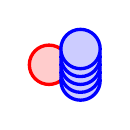
\begin{tikzpicture}[rotate=90, every node/.style={draw, very thick, circle, minimum width=0.5cm}]
                \node[red, fill=red!20!white] at (3, 0) (nd0) {};
                \foreach \i in {1,2,3,4,5} {
                    \node[blue, fill=blue!20!white] at (\i, -4) (nd1-\i) {};
                }
            \end{tikzpicture}
        \end{center}
    \end{figure}
\end{frame}

\begin{frame}{\ctitle{「代理人」}}
    \only<1> {
        \begin{figure}[h!]
            \begin{center}
                \begin{tikzpicture}[rotate=90, every node/.style={draw, very thick, circle, minimum width=0.5cm}]
                    \node[red, fill=red!20!white] at (3, 0) (nd0) {};
                    \foreach \i in {1,2,3,4,5} {
                        \node[blue, fill=blue!20!white] at (\i, -4) (nd1-\i) {};
                        \draw[->, very thick, >={Stealth}, red] (nd0) -- (nd1-\i);
                    }
                    \draw[draw=none] (nd0) -- node[red, draw=none, midway, anchor=north east]{$w$} (nd1-1);
                \end{tikzpicture}
            \end{center}
        \end{figure}
    
        注意到,建出來每一條邊都長得一模一樣
    }

    \only<2> {
        \begin{figure}[h!]
            \begin{center}
                \begin{tikzpicture}[rotate=90, every node/.style={draw, very thick, circle, minimum width=0.5cm}]
                    \node[red, fill=red!20!white] at (0, 0) (nd0-1) {};
                    \node[red, fill=red!20!white] at (3, 0) (nd0-2) {};
                    \node[red, fill=red!20!white] at (6, 0) (nd0-3) {};
                    \foreach \i in {1,2,3,4,5} {
                        \node[blue, fill=blue!20!white] at (\i, -4) (nd1-\i) {};
                        \draw[->, very thick, >={Stealth}, red] (nd0-1) -- (nd1-\i);
                        \draw[->, very thick, >={Stealth}, red] (nd0-2) -- (nd1-\i);
                        \draw[->, very thick, >={Stealth}, red] (nd0-3) -- (nd1-\i);
                    }
                \end{tikzpicture}
            \end{center}
        \end{figure}
    }
    
    \only<3> {
        一次詢問建出太多邊了

        \begin{figure}[h!]
            \begin{center}
                \begin{tikzpicture}[rotate=90, every node/.style={draw, very thick, circle, minimum width=0.5cm}]
                    \node[red, fill=red!20!white] at (3, 0) (nd0) {};
                    \node[blue, fill=cyan!50!white] at (3, -3) (nd2) {};
                    \foreach \i in {1,2,3,4,5} {
                        \node[blue, fill=blue!20!white] at (\i, -4) (nd1-\i) {};
                        \draw[->, very thick, >={Stealth}, blue] (nd2) -- (nd1-\i);
                    }
                    \draw[->, very thick, >={Stealth}, red] (nd0) -- node[draw=none, midway, anchor=north east]{$w$} (nd2);
                    \draw[blue, draw=none] (nd2) -- node[draw=none, midway, anchor=north east]{$0$} (nd1-1);
                \end{tikzpicture}
            \end{center}
        \end{figure}
    
        先建一個中間點,中間點再連藍色點\\
        詢問的時候,紅色點連\yum{一條邊}到中間點
    }
    
    \only<4> {
        \begin{figure}[h!]
            \begin{center}
                \begin{tikzpicture}[rotate=90, every node/.style={draw, very thick, circle, minimum width=0.5cm}]
                    \node[red, fill=red!20!white] at (1, 0) (nd0-1) {};
                    \node[red, fill=red!20!white] at (2, 0) (nd0-2) {};
                    \node[red, fill=red!20!white] at (3, 0) (nd0-3) {};
                    \node[red, fill=red!20!white] at (4, 0) (nd0-4) {};
                    \node[red, fill=red!20!white] at (5, 0) (nd0-5) {};
                    \node[blue, fill=cyan!50!white] at (3, -3) (nd2) {};
                    \foreach \i in {1,2,3,4,5} {
                        \node[blue, fill=blue!20!white] at (\i, -4) (nd1-\i) {};
                        \draw[->, very thick, >={Stealth}, blue] (nd2) -- (nd1-\i);
                        \draw[->, very thick, >={Stealth}, red] (nd0-\i) -- (nd2);
                    }
                \end{tikzpicture}
            \end{center}
        \end{figure}
    }

    \only<5> {
        以鬆弛的角度來說,連 $(a, b)$ 邊權 $w$,造成 $d(a) + w \ge d(b)$

        $a$ 連中間人 $c$,$d(a) + w \ge d(c)$ \\
        中間人 $c$ 連 $b_i$,$d(c) + 0 \ge d(b_i)$ \\
        $\Longrightarrow$ 實質上等同 $a$ 連 $b_i$,$d(a) + w \ge d(b_i)$
    }

\end{frame}

\begin{frame}{\ectitle}
    回到原本的問題,每次詢問要連邊的區間不一樣,每次開新的中間點的話問題沒有半點解決

    如果可以預先決定少少的中間點,每個中間點連到一個區間?\\
    如果可以預先決定一些區間,讓每個詢問都可以被這些區間拆分成少少段?

    \only<2> {
        把中間點開成\yum{線段樹}的樣子
    }
\end{frame}

\begin{frame}{\ectitle}
    \only<1> {
    \begin{figure}[h!]
        \begin{center}
            \begin{tikzpicture}[
                seg/.style={draw, very thick, rectangle, minimum width=0.5cm, anchor=north west},
                arrow/.style={->, very thick, >={Stealth}, blue},
                bluearr/.style={->, very thick, >={Stealth}, red},
                ndblue/.style={blue, fill={blue!20!white}},
                ndcyan/.style={blue, fill={cyan!50!white}},
                ndwhite/.style={blue, fill={white}},
            ]
                \node[anchor=center, draw, very thick, red, circle, fill=red!20!white] at (-3, -3.4) (nd-qry) {};

                \node[seg, ndwhite, minimum height=5.4cm] (nd-0) at (0, -0.7) {};
                \node[seg, ndwhite, minimum height=2.6cm] (nd-1) at (1, -0.7) {};
                \node[seg, ndwhite, minimum height=1.2cm] (nd-3) at (2, -0.7) {};
                \node[seg, ndblue, minimum height=0.5cm] (nd-7) at (3, -0.7) {1};
                \node[seg, ndblue, minimum height=0.5cm] (nd-8) at (3, -1.4) {2};
                \node[seg, ndwhite, minimum height=1.2cm] (nd-4) at (2, -2.1) {};
                \node[seg, ndblue, minimum height=0.5cm] (nd-9) at (3, -2.1) {3};
                \node[seg, ndblue, minimum height=0.5cm] (nd-10) at (3, -2.8) {4};
                \node[seg, ndwhite, minimum height=2.6cm] (nd-2) at (1, -3.5) {};
                \node[seg, ndwhite, minimum height=1.2cm] (nd-5) at (2, -3.5) {};
                \node[seg, ndblue, minimum height=0.5cm] (nd-11) at (3, -3.5) {5};
                \node[seg, ndblue, minimum height=0.5cm] (nd-12) at (3, -4.2) {6};
                \node[seg, ndwhite, minimum height=1.2cm] (nd-6) at (2, -4.9) {};
                \node[seg, ndblue, minimum height=0.5cm] (nd-13) at (3, -4.9) {7};
                \node[seg, ndblue, minimum height=0.5cm] (nd-14) at (3, -5.6) {8};
                \draw[arrow, blue] (nd-3) -- (nd-7);
                \draw[arrow, blue] (nd-3) -- (nd-8);
                \draw[arrow, blue] (nd-4) -- (nd-9);
                \draw[arrow, blue] (nd-4) -- (nd-10);
                \draw[arrow, blue] (nd-1) -- (nd-3);
                \draw[arrow, blue] (nd-1) -- (nd-4);
                \draw[arrow, blue] (nd-5) -- (nd-11);
                \draw[arrow, blue] (nd-5) -- (nd-12);
                \draw[arrow, blue] (nd-6) -- (nd-13);
                \draw[arrow, blue] (nd-6) -- (nd-14);
                \draw[arrow, blue] (nd-2) -- (nd-5);
                \draw[arrow, blue] (nd-2) -- (nd-6);
                \draw[arrow, blue] (nd-0) -- (nd-1);
                \draw[arrow, blue] (nd-0) -- (nd-2);
            \end{tikzpicture}
        \end{center}
    \end{figure}
    }

    \only<2> {
    \begin{figure}[h!]
        \begin{center}
            \begin{tikzpicture}[
                seg/.style={draw, very thick, rectangle, minimum width=0.5cm, anchor=north west},
                arrow/.style={->, very thick, >={Stealth}, blue},
                bluearr/.style={->, very thick, >={Stealth}, red},
                ndblue/.style={blue, fill={blue!20!white}},
                ndcyan/.style={blue, fill={cyan!50!white}},
                ndwhite/.style={blue, fill={white}},
                ndgray/.style={gray, fill={white}},
            ]
                \node[seg, ndgray, minimum height=5.4cm] (nd-0) at (0, -0.7) {};\node[seg, ndgray, minimum height=2.6cm] (nd-1) at (1, -0.7) {};\node[seg, ndgray, minimum height=1.2cm] (nd-3) at (2, -0.7) {};\node[seg, ndgray, minimum height=0.5cm] (nd-7) at (3, -0.7) {1};\node[seg, ndgray, minimum height=0.5cm] (nd-8) at (3, -1.4) {2};\node[seg, ndwhite, minimum height=1.2cm] (nd-4) at (2, -2.1) {};\node[seg, ndblue, minimum height=0.5cm] (nd-9) at (3, -2.1) {3};\node[seg, ndblue, minimum height=0.5cm] (nd-10) at (3, -2.8) {4};\node[seg, ndwhite, minimum height=2.6cm] (nd-2) at (1, -3.5) {};\node[seg, ndwhite, minimum height=1.2cm] (nd-5) at (2, -3.5) {};\node[seg, ndblue, minimum height=0.5cm] (nd-11) at (3, -3.5) {5};\node[seg, ndblue, minimum height=0.5cm] (nd-12) at (3, -4.2) {6};\node[seg, ndwhite, minimum height=1.2cm] (nd-6) at (2, -4.9) {};\node[seg, ndblue, minimum height=0.5cm] (nd-13) at (3, -4.9) {7};\node[seg, ndblue, minimum height=0.5cm] (nd-14) at (3, -5.6) {8};
                \draw[arrow, gray] (nd-3) -- (nd-7);\draw[arrow, gray] (nd-3) -- (nd-8);\draw[arrow, blue] (nd-4) -- (nd-9);\draw[arrow, blue] (nd-4) -- (nd-10);\draw[arrow, gray] (nd-1) -- (nd-3);\draw[arrow, gray] (nd-1) -- (nd-4);\draw[arrow, blue] (nd-5) -- (nd-11);\draw[arrow, blue] (nd-5) -- (nd-12);\draw[arrow, blue] (nd-6) -- (nd-13);\draw[arrow, blue] (nd-6) -- (nd-14);\draw[arrow, blue] (nd-2) -- (nd-5);\draw[arrow, blue] (nd-2) -- (nd-6);\draw[arrow, gray] (nd-0) -- (nd-1);\draw[arrow, gray] (nd-0) -- (nd-2);

                \node[anchor=center, draw, very thick, red, circle, fill=red!20!white] at (-3, -3.4) (nd-qry) {};
                \draw[arrow, red] (nd-qry) -- (nd-2);
                \draw[arrow, red] (nd-qry) -- (nd-4);
                \node[left of=nd-qry] {$[3, 8]$};
            \end{tikzpicture}
        \end{center}
    \end{figure}
    }

    \only<3> {
    \begin{figure}[h!]
        \begin{center}
            \begin{tikzpicture}[
                seg/.style={draw, very thick, rectangle, minimum width=0.5cm, anchor=north west},
                arrow/.style={->, very thick, >={Stealth}, blue},
                bluearr/.style={->, very thick, >={Stealth}, red},
                ndblue/.style={blue, fill={blue!20!white}},
                ndcyan/.style={blue, fill={cyan!50!white}},
                ndwhite/.style={blue, fill={white}},
                ndgray/.style={gray, fill={white}},
            ]
                \node[seg, ndgray, minimum height=5.4cm] (nd-0) at (0, -0.7) {};\node[seg, ndgray, minimum height=2.6cm] (nd-1) at (1, -0.7) {};\node[seg, ndgray, minimum height=1.2cm] (nd-3) at (2, -0.7) {};\node[seg, ndgray, minimum height=0.5cm] (nd-7) at (3, -0.7) {1};\node[seg, ndblue, minimum height=0.5cm] (nd-8) at (3, -1.4) {2};\node[seg, ndwhite, minimum height=1.2cm] (nd-4) at (2, -2.1) {};\node[seg, ndblue, minimum height=0.5cm] (nd-9) at (3, -2.1) {3};\node[seg, ndblue, minimum height=0.5cm] (nd-10) at (3, -2.8) {4};\node[seg, ndwhite, minimum height=2.6cm] (nd-2) at (1, -3.5) {};\node[seg, ndwhite, minimum height=1.2cm] (nd-5) at (2, -3.5) {};\node[seg, ndblue, minimum height=0.5cm] (nd-11) at (3, -3.5) {5};\node[seg, ndblue, minimum height=0.5cm] (nd-12) at (3, -4.2) {6};\node[seg, ndwhite, minimum height=1.2cm] (nd-6) at (2, -4.9) {};\node[seg, ndblue, minimum height=0.5cm] (nd-13) at (3, -4.9) {7};\node[seg, ndblue, minimum height=0.5cm] (nd-14) at (3, -5.6) {8};
                \draw[arrow, gray] (nd-3) -- (nd-7);\draw[arrow, gray] (nd-3) -- (nd-8);\draw[arrow, blue] (nd-4) -- (nd-9);\draw[arrow, blue] (nd-4) -- (nd-10);\draw[arrow, gray] (nd-1) -- (nd-3);\draw[arrow, gray] (nd-1) -- (nd-4);\draw[arrow, blue] (nd-5) -- (nd-11);\draw[arrow, blue] (nd-5) -- (nd-12);\draw[arrow, blue] (nd-6) -- (nd-13);\draw[arrow, blue] (nd-6) -- (nd-14);\draw[arrow, blue] (nd-2) -- (nd-5);\draw[arrow, blue] (nd-2) -- (nd-6);\draw[arrow, gray] (nd-0) -- (nd-1);\draw[arrow, gray] (nd-0) -- (nd-2);

                \node[anchor=center, draw, very thick, red, circle, fill=red!20!white] at (-3, -3.4) (nd-qry-1) {};
                \draw[arrow, red] (nd-qry-1) -- (nd-2);
                \draw[arrow, red] (nd-qry-1) -- (nd-4);
                \node[left of=nd-qry-1] {$[3, 8]$};
                
                \node[anchor=center, draw, very thick, red, circle, fill=red!20!white] at (-3, -1.4) (nd-qry-2) {};
                \draw[arrow, red] (nd-qry-2) -- (nd-4);
                \draw[arrow, red] (nd-qry-2) -- (nd-8);
                \node[left of=nd-qry-2] {$[2, 4]$};
                
                \node[anchor=center, draw, very thick, red, circle, fill=red!20!white] at (-3, -5.4) (nd-qry-3) {};
                \draw[arrow, red] (nd-qry-3) -- (nd-13);
                \node[left of=nd-qry-3] {$[7, 7]$};
                
            \end{tikzpicture}
        \end{center}
    \end{figure}
    }
\end{frame}

\begin{frame}{\ectitle}
    對一個線段樹節點連一條邊,等同於對區間內所有點分別連邊
    
    如果把整張圖反過來:從線段樹節點連出來,等同於從區間內所有點分別連出來
\end{frame}

\begin{frame}{\ectitle}
    預先建兩棵線段樹,一棵從根往葉子連邊,一棵從葉子往根連邊 \\
    每次詢問根據方向在對應的樹上連 $O(\log N)$ 條邊,就可以建出一樣的圖(在最短路的意義上一樣)

    單源最短路?dijkstra 就好
\end{frame}

\begin{frame}{\ectitle}
    最後建出來的圖上:
    \begin{itemize}
        \item 一棵線段樹有 $2N$ 個節點,但是兩棵線段樹葉節點可以共用,總共 $3N$ 個點
        \item 兩棵線段樹各建 $O(N)$ 條邊,之後每個詢問建 $O(\log N)$ 條邊,總共 $O(N + Q \log N)$ 條邊
    \end{itemize}
    時間複雜度 $O((N + Q \log N) \log N)$
\end{frame}

\begin{frame}{\ectitle}
    線段樹本身和我們是怎麼建圖的並\yum{沒有}關係 \\
    我們甚至可以用 sparse table 建類似的圖

    線段樹在這裡發揮的最大價值是\yum{把詢問區間拆解}成一些特別的小區間
\end{frame}


